\documentclass{beamer} % [hyperref={colorlinks = true,	urlcolor=blue}]
\usetheme{metropolis}           % Use metropolis theme
%\usepackage[german]{babel}  
\usepackage[utf8]{inputenc}	%dt Sonderzeichen wie ß
\usepackage{tikz}
\usepackage{amssymb}
\usepackage{multirow}
\usepackage{pgfpages}
\usepackage{cite}
\usepackage{graphicx}
\usepackage{animate}

\usepackage{multimedia}
\usepackage{subfig}

\usepackage{booktabs}

%\setbeameroption{show notes on second screen=right}  %% Uncomment this to get Notes


%\renewcommand*{\figurename}{Abb.}
\setbeamertemplate{frame footer}{\textit{Drift Detection in Text Data with Document Embeddings}, Feldhans et al.}

%Acknowledgments This work has been supported by the German Federal Ministry of Education and Research (BMBF) within the project EML4U under the grant no 01IS19080 A and B.

\title{Drift Detection in Text Data with Document Embeddings}
%\date{25.11.2021}
\author{\textbf{Robert Feldhans}\textsuperscript{1},
	Adrian Wilke\textsuperscript{2},
	Stefan Heindorf\textsuperscript{2}, 
	Mohammad Hossein Shaker\textsuperscript{3}, 
	Barbara Hammer\textsuperscript{1}, 
	Axel-Cyrille Ngonga Ngomo\textsuperscript{2}, 
	Eyke Hüllermeier\textsuperscript{3}
} % change accordingly
\institute{\textsuperscript{1} Bielefeld University, Germany\\
\textsuperscript{2} DICE group, Paderborn University, Germany\\
\textsuperscript{3} University of Munich (LMU), Germany\\

This work has been supported by the German Federal Ministry of Education and Research (BMBF) within the project EML4U under the grant no 01IS19080 A and B.
}

\begin{document}
	\maketitle
	
	
	\begin{frame}{Drift in general}
		\begin{alertblock}{Description}
			\begin{itemize}
				\item In practice, data fed into ML models often evolves over time
				\item E.g. inflation has impact on credit scoring, climate change has impact on weather forecasting
			\end{itemize}
		\end{alertblock}
		\pause
		\begin{alertblock}{Problems}
			\begin{itemize}
				\item Drift causes performance degradation
				\item Retraining models is costly and should be avoided
				\item Detection methods oftentimes assume input data to be low-dimensional, hand-engineered vector space
			\end{itemize}
		\end{alertblock}
	\end{frame}

	\begin{frame}{Drift in NLP - Document embeddings}
		\begin{alertblock}{Special properties}
			\begin{itemize}
				\item Medium to high dimensionality (standard BERT has 768)
				\item One of the most prominent metrics is cosine similarity
			\end{itemize}
		\end{alertblock}
		\pause
		\begin{alertblock}{Research Questions}
			\begin{enumerate}
				\item[RQ1] Which drift detector works best for document embeddings?
				\item[RQ2] How does the performance of a drift detector depend on the embedding
				dimensions?
			\end{enumerate}
		\end{alertblock}
	
	\end{frame}

	\begin{frame}{Algorithms}
		\begin{alertblock}{Kolmogorov-Smirnov (KS)}
			\vspace{0.1cm}\hspace{1cm} Statistical independence test based on maximum absolute difference
		\end{alertblock}
	
		\begin{alertblock}{Kernel Two-Sample (KTS)}
			\vspace{0.1cm}\hspace{1cm} Statistical independence test based on
Maximum Mean Discrepancy (MMD)
		\end{alertblock}
	
		\begin{alertblock}{Least-Squares Density Difference (LSDD)}
			\vspace{0.1cm}\hspace{1cm} Based on least-squares
density difference estimation
method
		\end{alertblock}
	
		\begin{alertblock}{Confidence Distribution Batch Detection (CDBD)}
			\vspace{0.1cm}\hspace{1cm} Uncertainty-based semi-supervised
		\end{alertblock}
	\end{frame}

	\begin{frame}{Datasets}
		
		\begin{alertblock}{Amazon movie reviews}
			\begin{itemize}
				\item Amazon reviews of movies, sentiment expressed by label of one to five stars
			\end{itemize}
		\end{alertblock}
	
		\begin{alertblock}{Twitter election}
			\begin{itemize}
				\item Tweets which contain $\#Biden$ or $\#Trump$ from around the time of the 2020 US election
				\item Real world drift occurrence in $t_{debate}$ and $t_{election}$
			\end{itemize}
		\end{alertblock}
	\end{frame}

	\begin{frame}{Evaluation Setup: Sampling}
		\begin{alertblock}{Drift Induction}
			\begin{itemize}
				\item Negative adjectives are added step-wise to randomly chosen data points of one of the test sets
				\item In each step, an additional 5\% of the data points are altered
				\item $\Rightarrow$ Test how fast a gradual drift is detected
			\end{itemize}
		\end{alertblock}
	
		\begin{alertblock}{Same Distribution}
			\begin{itemize}
				\item Two subsets are created, both are of the same distribution in terms of creation time, class balance, size
				\item $\Rightarrow$ Test whether drift detectors abstain
from identifying drift where there is none
			\end{itemize}
		\end{alertblock}
	\end{frame}
	
	\begin{frame}{Evaluation Setup: Sampling II}
		\begin{alertblock}{Different Classes}
			\begin{itemize}
				\item Two subsets are created, both only contain samples of one class, i.e. one star vs five star reviews and tweets containing $\#Biden$ vs $\#Trump$
				\item $\Rightarrow$ Establish maximum possible (virtual) drift and give context to Drift induction experiment
			\end{itemize}
		\end{alertblock}
	
		\begin{alertblock}{Different Distribution (only Twitter)}
			\begin{itemize}
				\item Apply prior knowledge of Twitter dataset and check for drift between two baselines as well as $t_{debate}$ and $t_{election}$
				\item $\Rightarrow$ Test algorithms in a real world scenario
			\end{itemize}
		\end{alertblock}
	\end{frame}

	\begin{frame}{Embedding Models}
		\begin{alertblock}{BERT}
			\begin{itemize}
				\item Produces embeddings with 768 dimensions
				\item Retrained for the Amazon dataset on the Amazon dataset
				\item Not retrained on Twitter dataset
			\end{itemize}
		\end{alertblock}
	
		\begin{alertblock}{Word2Vec}
			\begin{itemize}
				\item Two distinct models, produce embeddings with 50 and 768 dimensions
				\item Trained from scratch on both datasets
			\end{itemize}
		\end{alertblock}
	\end{frame}

	{
	\setbeamertemplate{frame footer}{}
	\begin{frame}{Results: Drift Injection}
		\begin{figure}[htb!] % [H] [ht!]
			\centering
			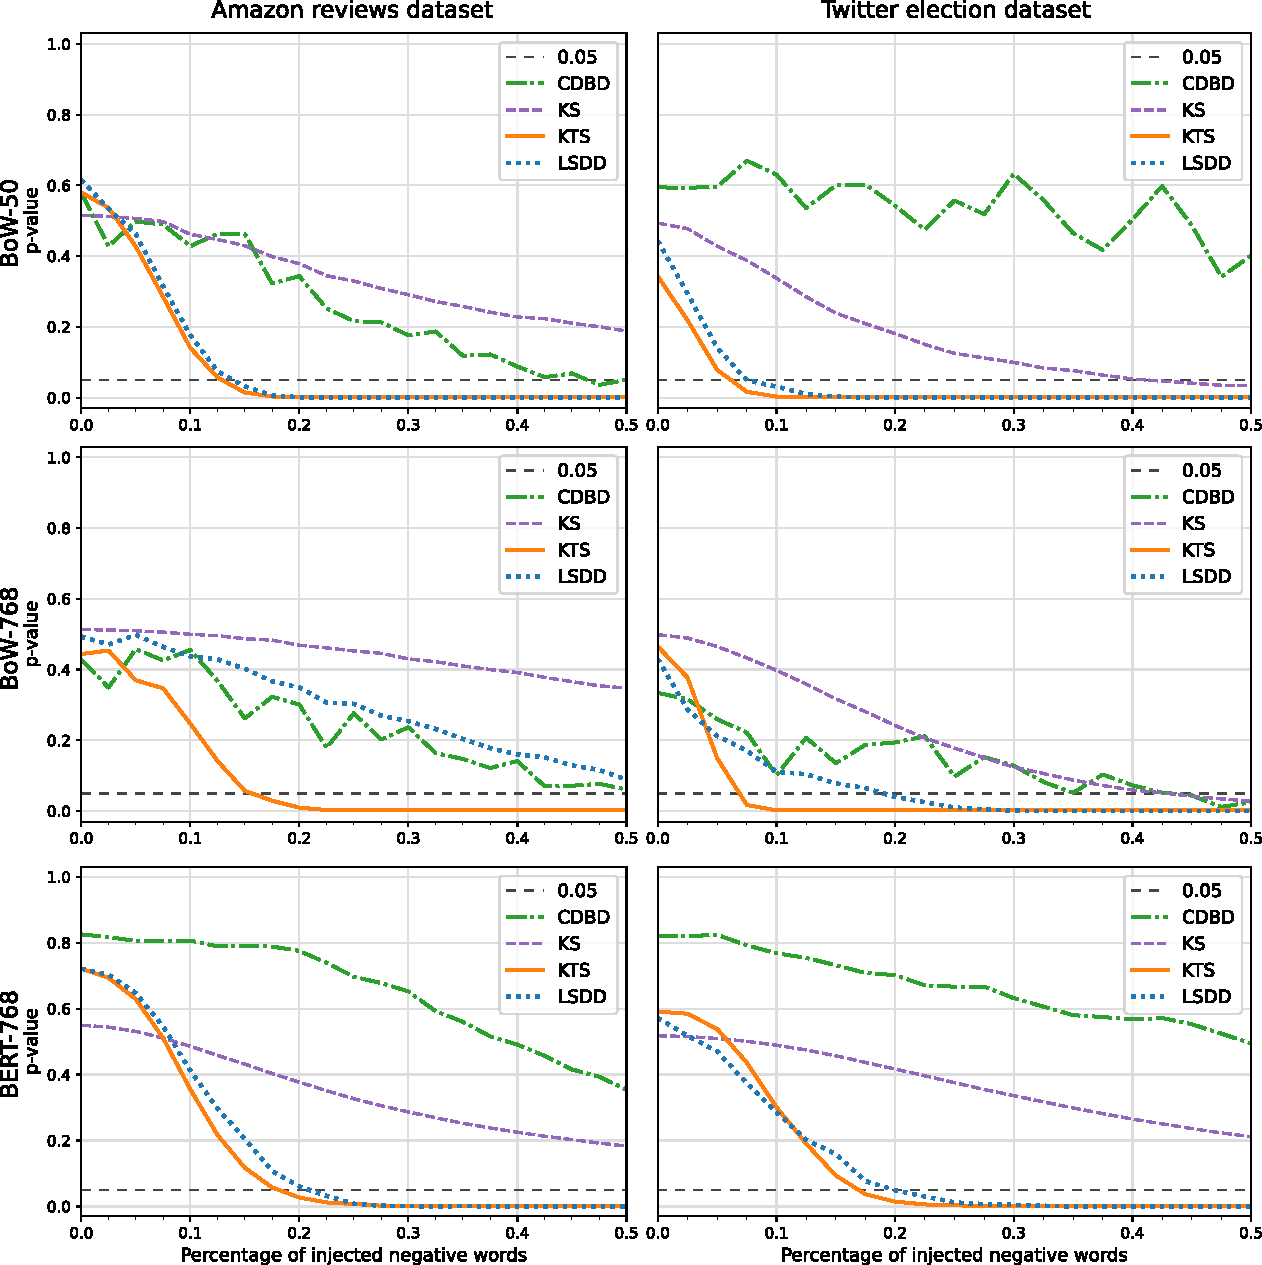
\includegraphics[width=.75\textwidth]{Bilder/drift_induction_all.pdf}
			%\vspace{-0.5cm}
			%\caption{Drift detection results on injection experiments.
			%	Presented is the mean p-value of all runs.
				%Cosine similarity is displayed directly, other results are p-values.
			%}
			\label{Fig:drift_induction_all}
		\end{figure}
	\end{frame}
	}

	\begin{frame}{Results: Same Distribution}
		\begin{alertblock}{Results of the Same Distribution experiment}
			\begin{itemize}
				\item CDBD generally performs best ($p \approx 0.7$)
				\item KS detector performs very consistently ($p \approx 0.5$)
				\item KTS and LSDD have high standard deviation, and feature the single best and worst result, but generally lie between KS and CDBD
			\end{itemize}
		\end{alertblock}
		$\Rightarrow$ Regarding \alert{\textbf{RQ2}}, we do not see a consistent effect of the
		embedding dimension
	\end{frame}
	
	\begin{frame}{Results: Different Classes}
		\begin{alertblock}{Results of the Different Classes experiment}
			\begin{itemize}
				\item KTS and LSDD very confident in detecting drift
				\item KS struggles detecting this kind of drift, especially in the Twitter dataset and more so with data of 768 dimensions 
			\end{itemize}
		\end{alertblock}
		$\Rightarrow$ CDBD detector was omitted as it did not fit this specific experiment setup
	\end{frame}
	
	\begin{frame}{Results: Twitter Different Distribution}
		\begin{figure}[htb!] % [H] [ht!]
			\centering
			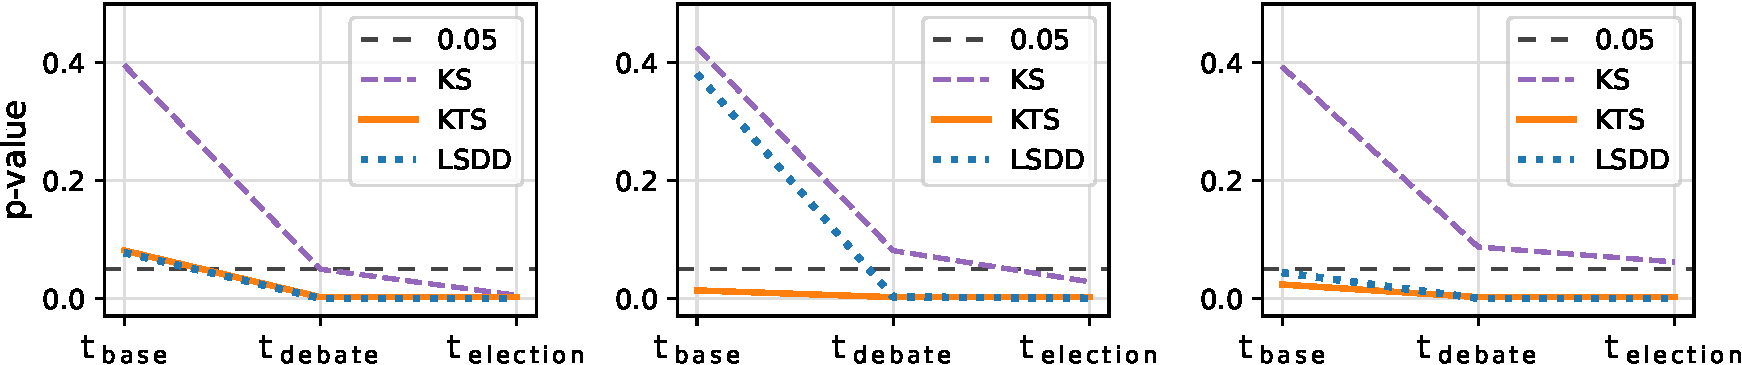
\includegraphics[width=\textwidth]{Bilder/diff_dist_all}
			%\vspace{-0.5cm}
			\caption{Results of Twitter different distribution experiment (mean p-value of all runs):
				BoW-50 (left), BoW-768 (center) and BERT-768 (right)}
			\label{Fig:diff_dist_all}
		\end{figure}
	\end{frame}

	\begin{frame}{Conclusion}
		\begin{alertblock}{RQ1}
			\begin{itemize}
				\item LSDD and KTS best Drift detectors, LSDD better on real-world Twitter experiment
				\item KS average with conservative  estimation  of  p-values
				\item CDBD requires a large reference batch to produce robust results, questioning its usefulness in many practical applications
			\end{itemize}
		\end{alertblock}
		
		\begin{alertblock}{RQ2}
			\begin{itemize}
				\item Lower embedding dimensions tend to produce better drift detection results
			\end{itemize}
		\end{alertblock}
	\end{frame}


	\begin{frame}[standout]
		Questions?
	\end{frame}

	\appendix
	
	\begin{frame}{Twitter breakdown}
		\begin{figure}[htb!] % [H] [ht!]
			\centering
			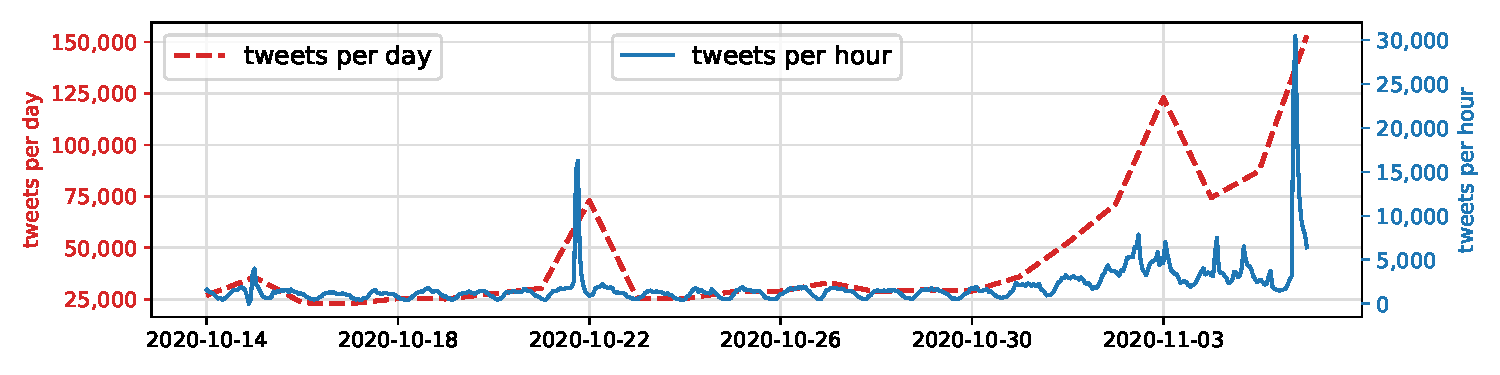
\includegraphics[width=.98\linewidth]{Bilder/tweet_counts.pdf}
			%\vspace{-0.4cm}
			\caption{Amount of tweets in the Twitter election dataset by day (red) and hour (blue).
				Note the sharp spike during the last TV debate ($t_{\mathit{debate}} = $ 2020-10-22) and the overall increase during the election day ($t_{\mathit{election}} = $ 2020-11-03).
				Slight inaccuracies in the timeline can be attributed to time zone-related shifts.}
			\label{Fig:tweet_counts}
		\end{figure}
	\end{frame}
	
	
	
\end{document}
	
	
	